\documentclass{article}
\usepackage[a4paper,margin=0.1 cm,portrait]{geometry}
\usepackage{graphicx}
\usepackage{caption}
\usepackage{subcaption}
\usepackage{float}
\usepackage{booktabs}
\usepackage{tabularx}
\usepackage{ragged2e}
\setlength{\tabcolsep}{0.0\textwidth}
\begin{document}
\centering
\begin{center}

\begin{tabularx}{1\textwidth}{cc}
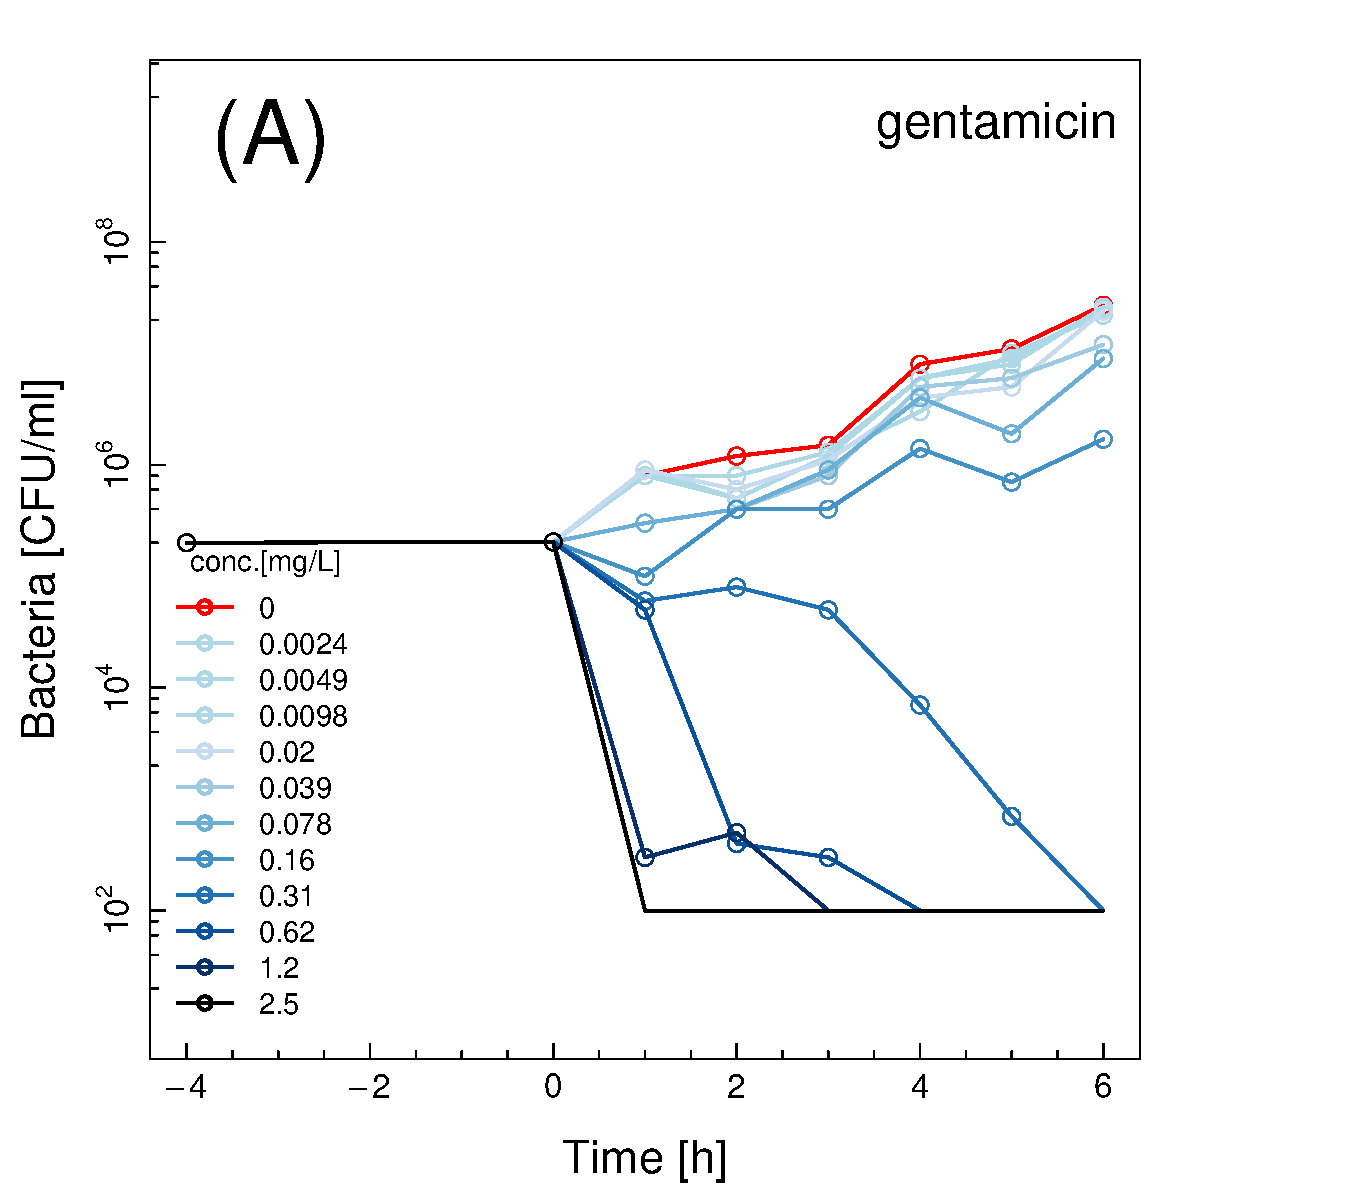
\includegraphics[trim = 0mm 0mm 0mm 0mm, clip,width=0.35\textwidth]{WT_Genregression} & 
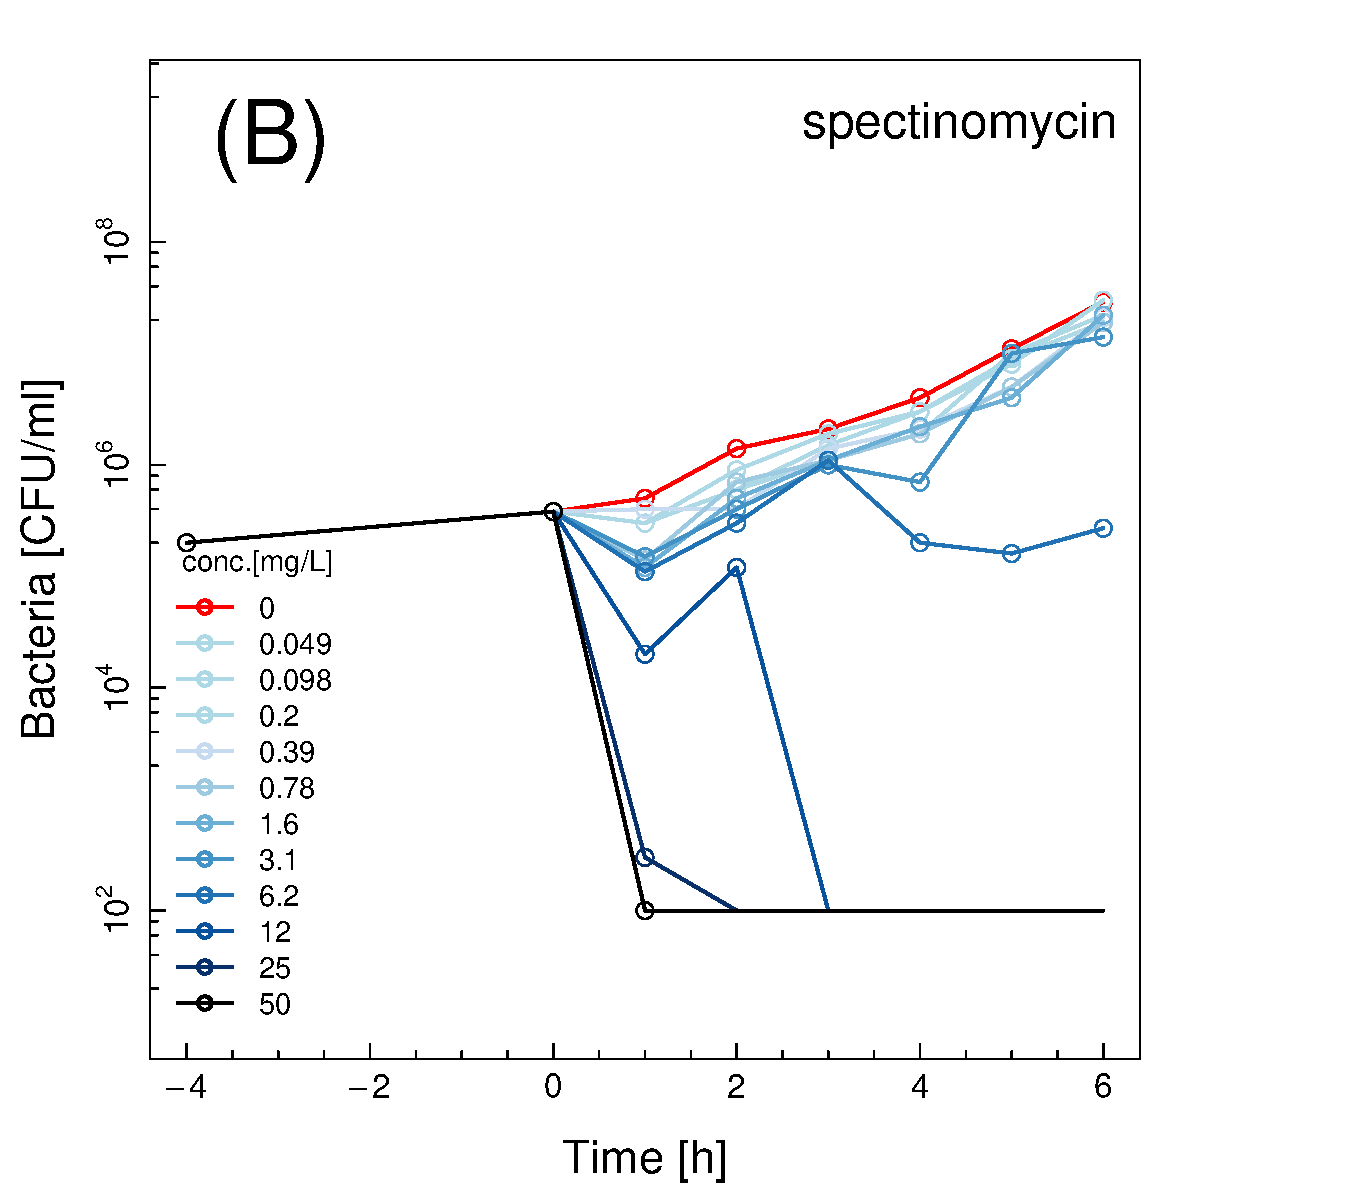
\includegraphics[trim = 0mm 0mm 0mm 0mm, clip,width=0.35\textwidth]{WT_Specregression} \\
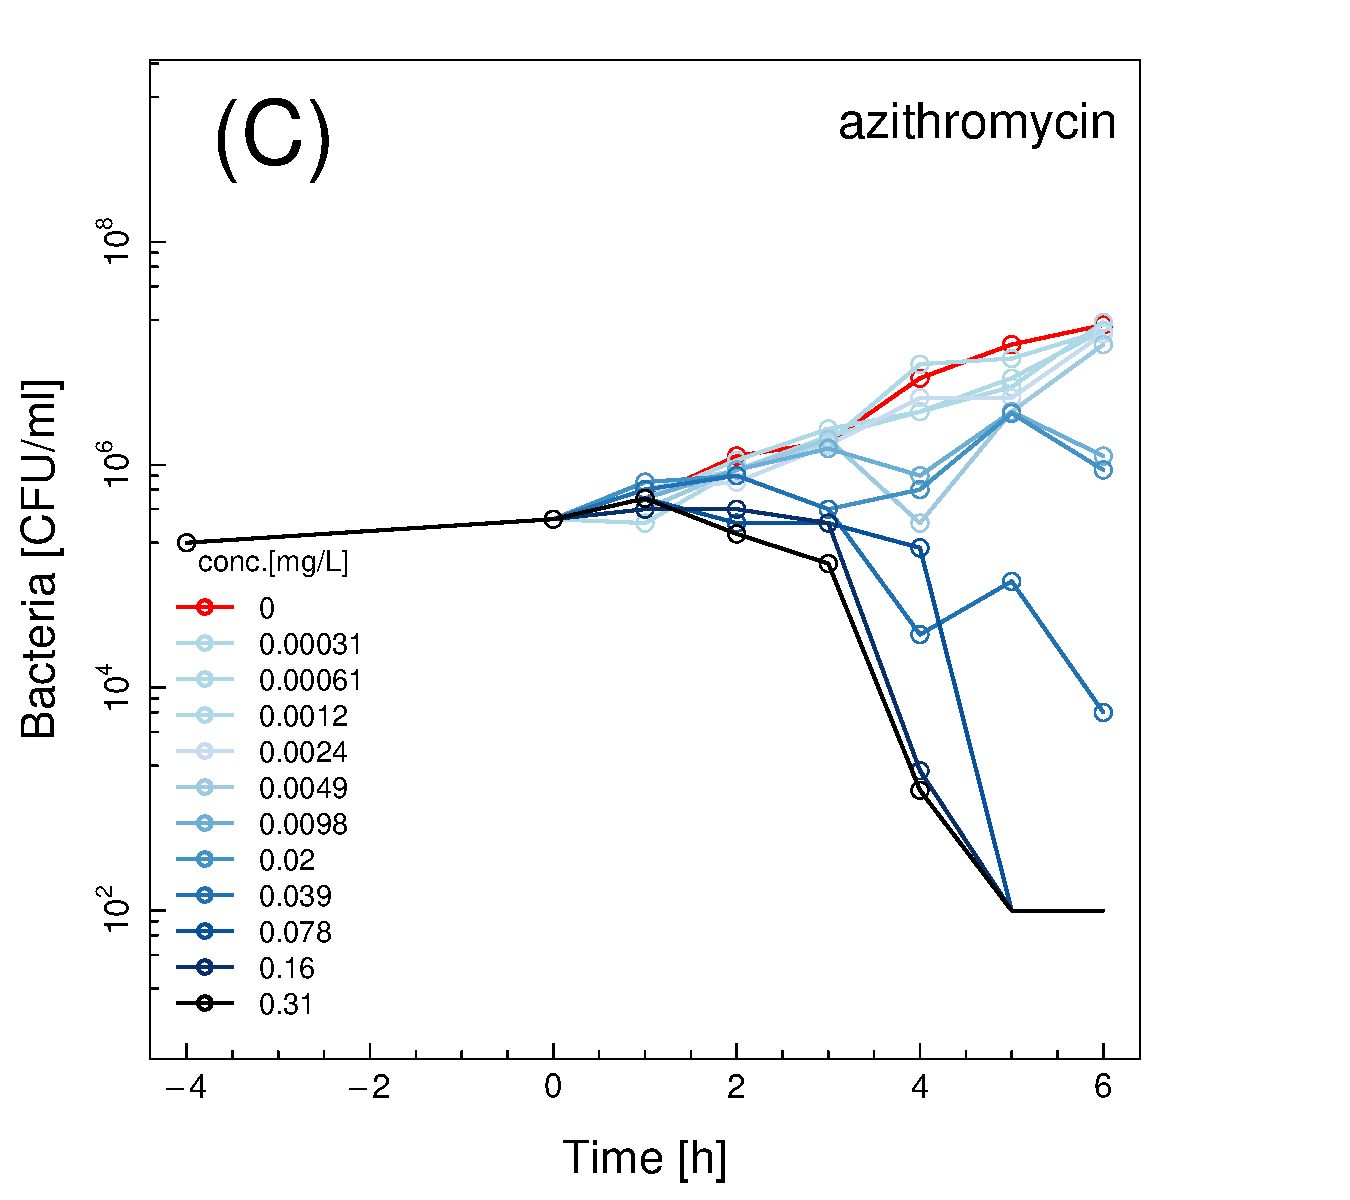
\includegraphics[trim = 0mm 0mm 0mm 0mm, clip,width=0.35\textwidth]{WT_AZregression}  &
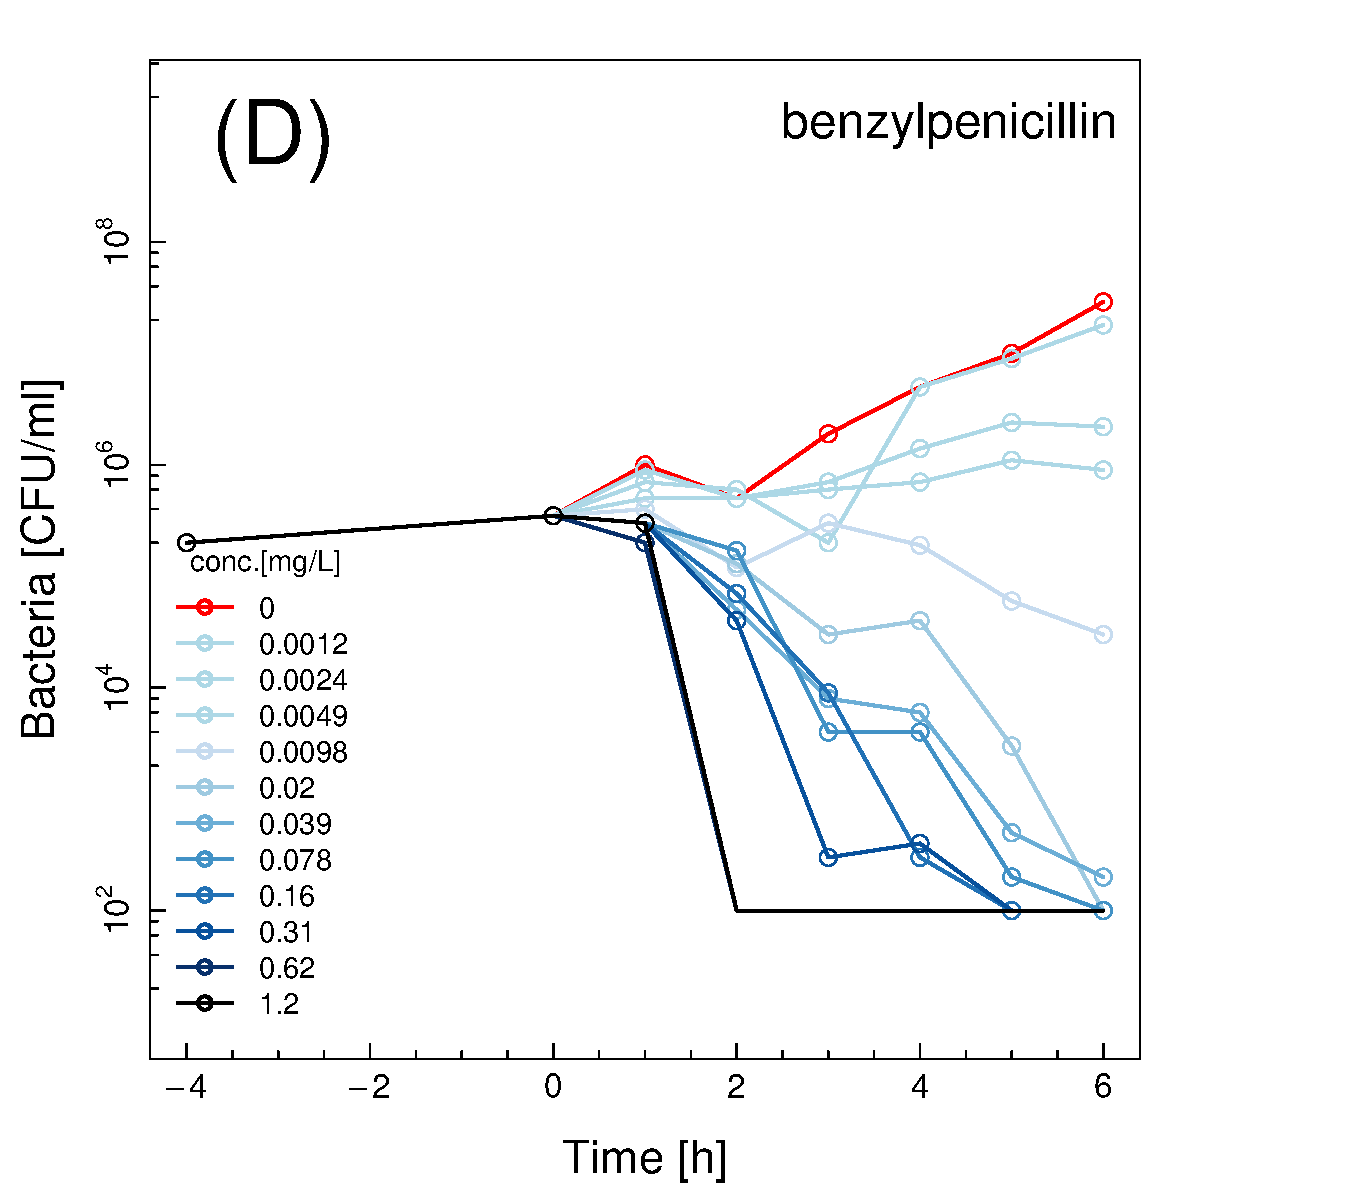
\includegraphics[trim = 0mm 0mm 0mm 0mm, clip,width=0.35\textwidth]{WT_Penregression}  \\
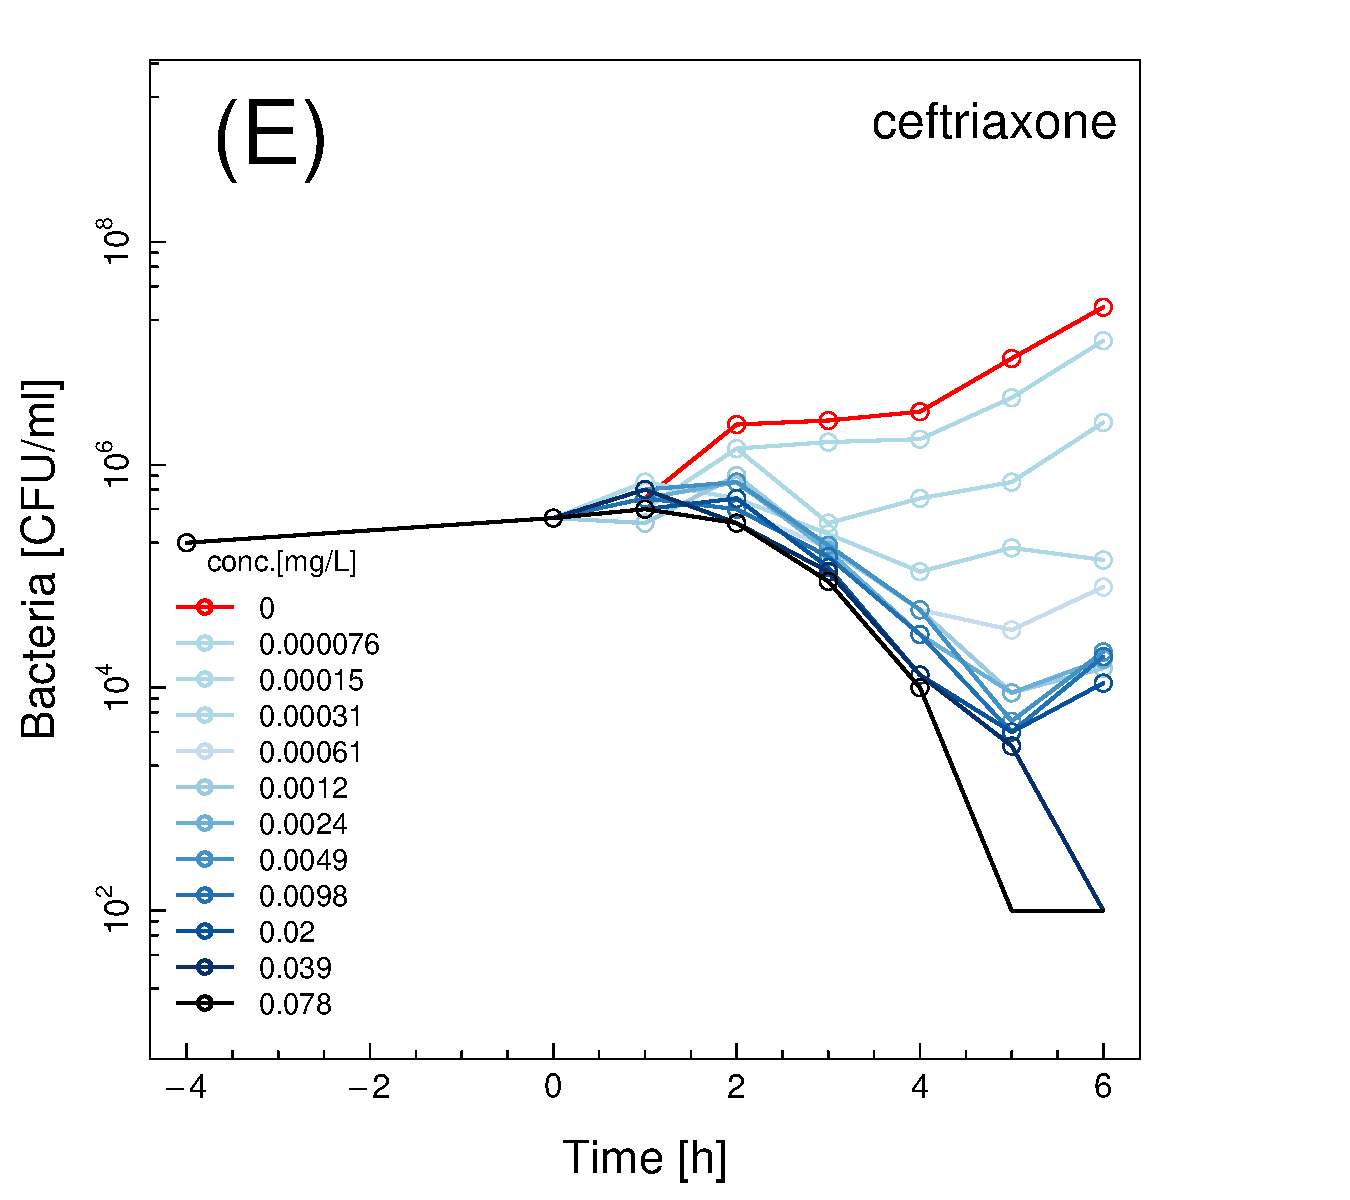
\includegraphics[trim = 0mm 0mm 0mm 0mm, clip,width=0.35\textwidth]{WT_CTregression}&  
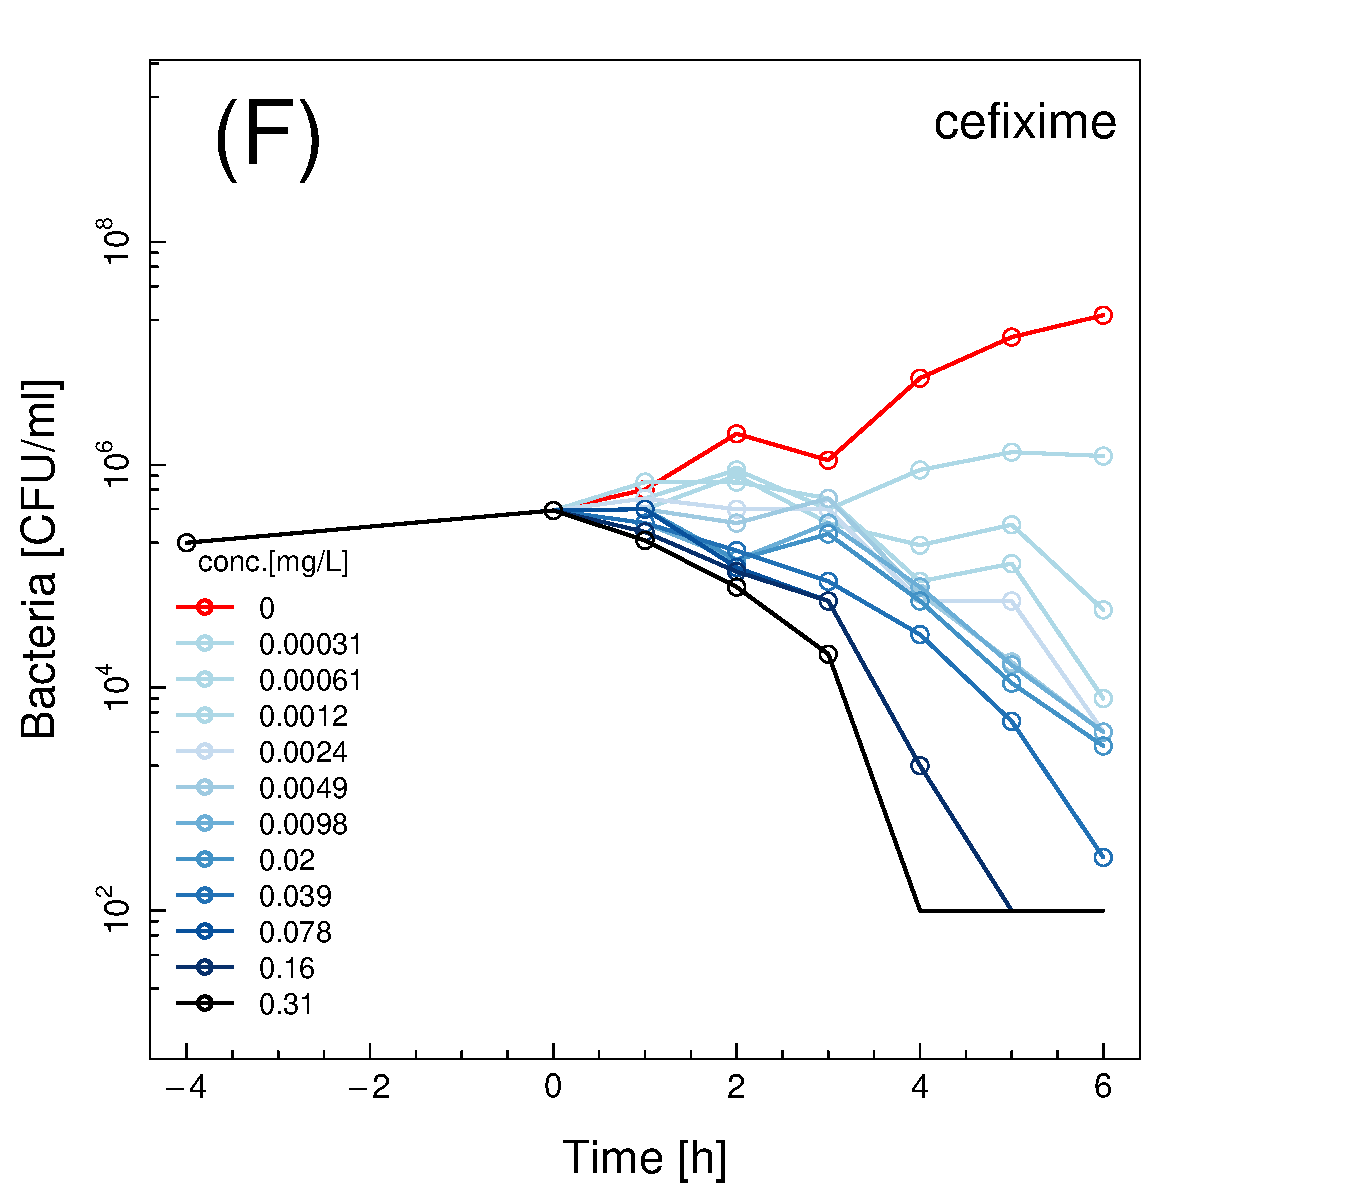
\includegraphics[trim = 0mm 0mm 0mm 0mm, clip,width=0.35\textwidth]{WT_CXregression}\\
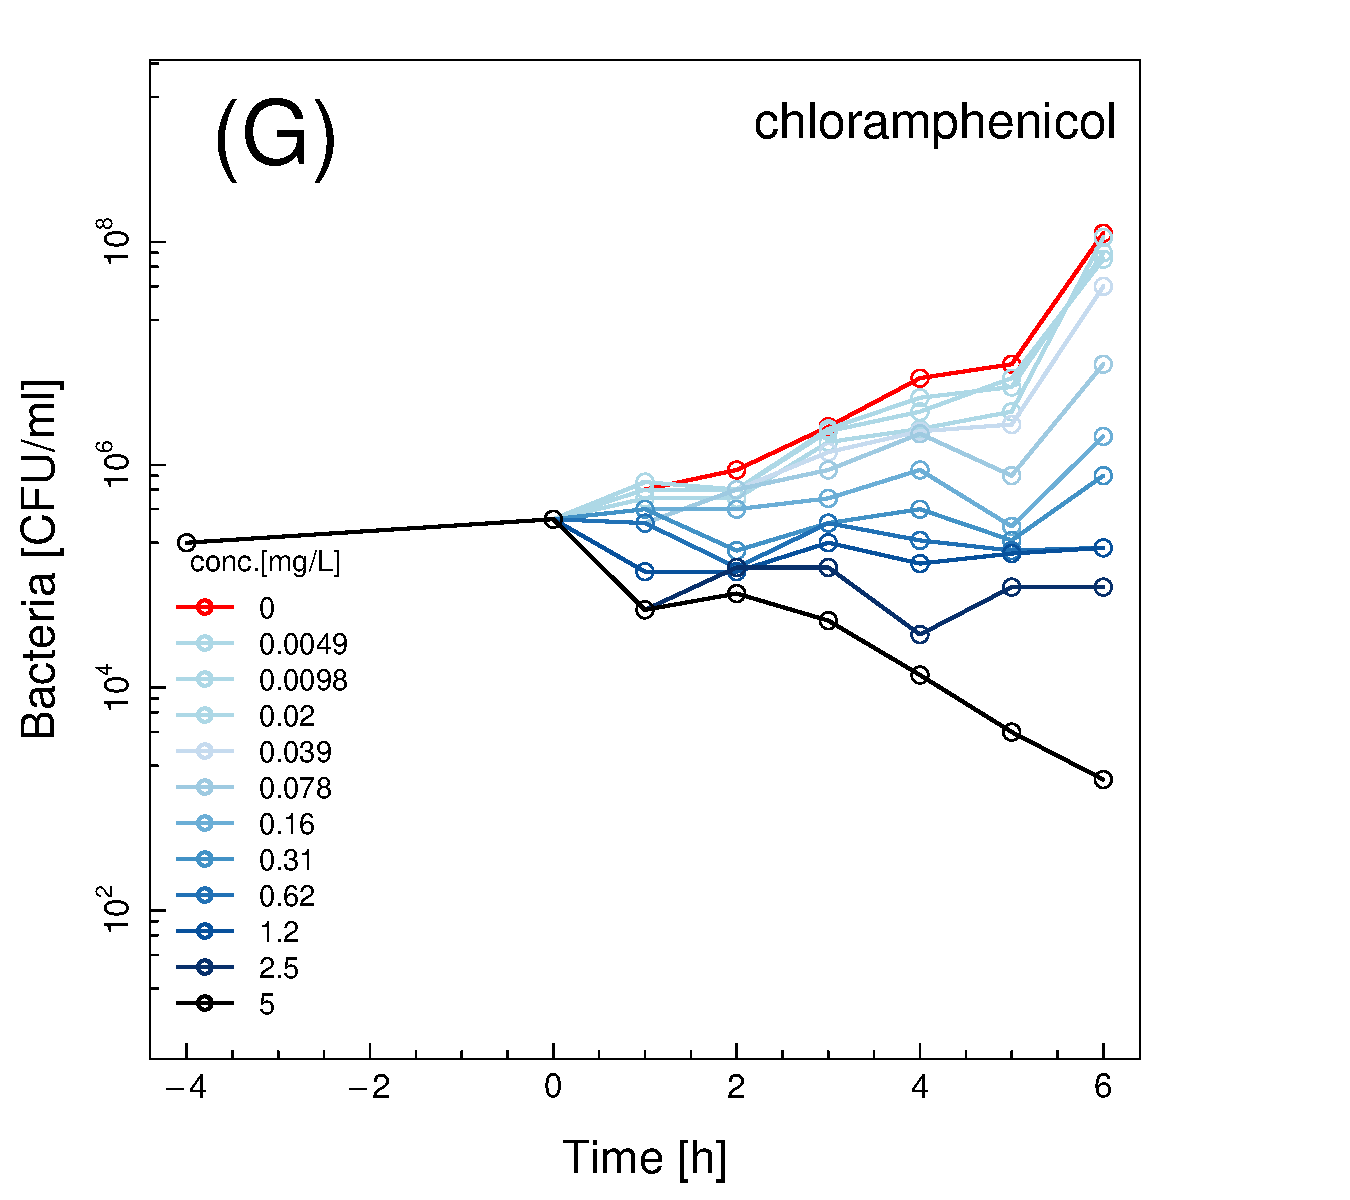
\includegraphics[trim = 0mm 0mm 0mm 0mm, clip,width=0.35\textwidth]{WT_Chlorregression} & 
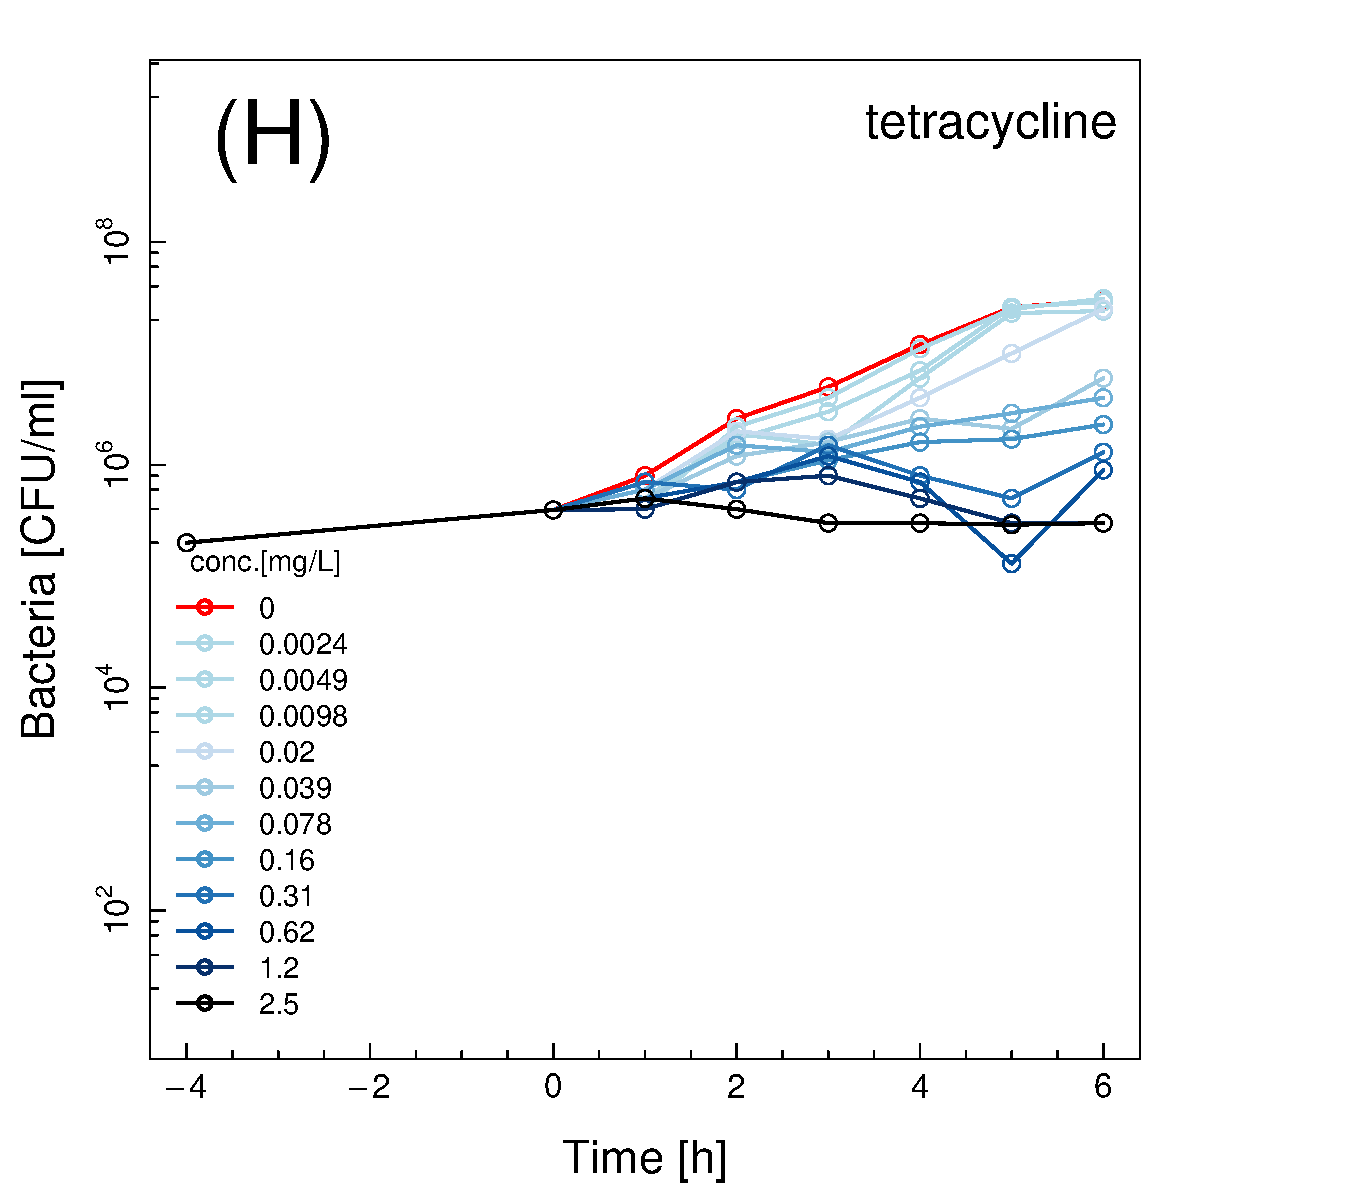
\includegraphics[trim = 0mm 0mm 0mm 0mm, clip,width=0.35\textwidth]{WT_Tetregression} \\  
\end{tabularx}
\end{center}
\end{document}